\documentclass[11pt, a4paper]{article} %twoside
\usepackage{wrapfig}
\usepackage{epigraph}
\usepackage{graphicx}
\usepackage[swedish]{babel}
\usepackage{enumitem}

\usepackage[hidelinks]{hyperref}
\usepackage[hyphens]{url}


\usepackage{setspace}
\onehalfspacing

\usepackage[font={small,it}]{caption}

\usepackage{etoolbox}
\AtBeginEnvironment{quote}{\small}

\usepackage{dirtytalk}

\usepackage[margin=3cm]{geometry}
\usepackage{float, blindtext, kantlipsum}

\usepackage[toc,page]{appendix}
\usepackage[section=subsection, toc, acronym, nonumberlist]{glossaries}
\renewcommand{\appendixtocname}{Bilagor} \renewcommand{\appendixpagename}{Bilagor}
\addto\captionsswedish{\renewcommand\appendixname{Bilagor}}

%\renewcommand{\thefootnote}{\alph{footnote}}

\newcommand{\symfootnote}[1]{%
\let\oldthefootnote=\thefootnote%
\stepcounter{mpfootnote}%
\addtocounter{footnote}{-1}%
\renewcommand{\thefootnote}{$\star$}%
\footnote{#1}%
\let\thefootnote=\oldthefootnote%
}

\usepackage[citestyle=verbose-ibid, bibstyle=authoryear, natbib=true, url=false, doi=false, isbn=false, backend=biber, labeldateparts]{biblatex}
\AtEveryBibitem{%
  \clearlist{language}%
  \clearfield{note}%
}

\DeclareSortingTemplate{mysort}{
  \sort{
	\field{editora}
  }
}

\renewbibmacro{in:}{}
\renewbibmacro{in:}{%
  \ifboolexpr{%
     test {\ifentrytype{article}}%
     or
     test {\ifentrytype{incollection}}%
  }{}{\printtext{\bibstring{in}\intitlepunct}}%
}

\DeclareBibliographyDriver{misc}{%
  \usebibmacro{bibindex}%
  \usebibmacro{begentry}%
  \usebibmacro{author}%
  \setunit{\labelnamepunct}\newblock
  \usebibmacro{maintitle+title}%
  \newunit
  \usebibmacro{date}%
  \usebibmacro{url+urldate}%
  \newunit\newblock
  \printfield{number}%
  \newunit
  %\usebibmacro{byeditor+others}%
  \setunit{=\addspace}
  \printfield{series}%
  \setunit{\adddot\addspace}
  \usebibmacro{publisher+location+date}%
  \newunit\newblock
  \usebibmacro{finentry}
}

\usepackage{xpatch}
\xpatchbibmacro{byeditor+othersstrg}{\printtext}{\printtext[parens]}{}{}


\renewbibmacro*{byeditor+others}{%
  \ifnameundef{editor}
    {}
    {\printnames[byeditor]{editor}%
     \setunit{\addspace}%
     \usebibmacro{byeditor+othersstrg}%
     \clearname{editor}%
     \newunit}%
  \usebibmacro{byeditorx}%
  \usebibmacro{bytranslator+others}
}

\DefineBibliographyStrings{swedish}{%
    byeditor = {red\adddot},%
}

\DeclareBibliographyDriver{audio}{%
  \printnames{editora}%
  \newunit 
  \printfield[parens]{year}%
  \newunit\newblock
  \printfield{title}%
    \newunit
  \usebibmacro{url+urldate}%
    \newunit\newblock
  \usebibmacro{publisher+location+date}%
  \finentry
}

\addbibresource{bibtex/kandidatarbete.bib}

\usepackage{csquotes}

\usepackage{sectsty}
\subsubsectionfont{\normalfont\itshape}
%\subsectionfont{\normalfont\centering}

\usepackage{titlesec}
\titleformat{\section}
  {\normalfont\LARGE\bfseries}{\thesection}{1em}{}[{}]

  \newcommand{\sectionbreak}{\clearpage}
  %\titlerule[0.8pt]

\makeglossaries

\newacronym{api}{API}{Application Programming Interface}
\newacronym{cgm}{CGM}{Continuous Glucose Monitor}
\newacronym{fgm}{FGM}{Flash Glucose Monitor}
\newacronym{pmson}{PMSon}{Parameter Mapping Sonification}
\newacronym{fifo}{FIFO}{First In, First Out}
\newacronym{vps}{VPS}{Virtual Private Server}
\newacronym{ux}{UX}{User Experience}
\newacronym{gdpr}{GDPR}{General Data Protection Regulation}

\setglossarystyle{long}

%\newglossaryentry{API}
%{
%    name=API,
%	description={Application Programming Interface.}
%}


\newglossaryentry{frontend}
{
    name=Front end,
	description={Användargränssnittet i webbutveckling}
}

\newglossaryentry{backend}
{
    name=Back end,
	description={Allt som rör sig ''under huven'', server-side programmering}
}

\newglossaryentry{supercollider}
{
    name=SuperCollider,
	description={Ett programmeringsspråk och plattform för syntes av ljud, och musikalisk programmering}
}

\newglossaryentry{ugen}
{
    name=\texttt{UGen},
	description={En komponent av SuperCollider som används som byggsten till \texttt{SynthDef}:ar}
}

\newglossaryentry{synthdef}
{
    name=\texttt{SynthDef},
	description={En komponent av SuperCollider för att formulera sammansättningar av synthar}
}

\newglossaryentry{pattern}
{
    name=\texttt{Pattern},
	description={Ett verktyg i SuperCollider för att formulera och generera musikaliska händelser}
}

\newglossaryentry{stack}
{
    name=Stack,
	description={Alla delar som utgör en plattform eller ett system}
}

\newglossaryentry{flask}
{
  name=Flask,
description={Ett Python-ramverk som används i webbutveckling}
}

\newglossaryentry{audification}
{
    name=Audifiering,
    text=audifiering,
	description={en. \emph{audification}. En typ av sonifiering. Direktöversättningen av en dataserie till ljudkurvor}
}

%\newglossaryentry{fifo}
%{
%    name=FIFO-system,
%	description={First in, First out. En typ av kösystem}
%}

\newglossaryentry{sonification}
{
    name=Sonifiering,
    text=sonifiering,
	description={en. \emph{sonification}. Gestaltningen eller representationen av en dataserie i ljud}
}

\newglossaryentry{mappning}
{
    name=Mappning,
	description={Ihopparningen av ett element (invariabel) till en annan (utvariabel)}
}

\newglossaryentry{parametermapping}
{
    name=Parameter Mapping Sonification,
	description={}
}

\usepackage[yyyymmdd]{datetime}
\renewcommand{\dateseparator}{--}

\begin{document}

\clearpage


\newpage

\renewcommand{\abstractname}{Tack}
\begin{abstract}
  \noindent
Stort tack till min texthandledare Kim Hedås och lärare Erik Peters för alla kloka råd och vägledning! Även stort tack till Herman Wikner\symfootnote{Hermans GitHub finns tillgänglig på: \url{https://github.com/hermanwikner} (hämtad \today).} som hjälpt mig bygga användargränssnittet i React.js! 
\end{abstract}
\thispagestyle{empty}
\clearpage

\pagenumbering{arabic}

\begin{singlespace}
  \tableofcontents
\end{singlespace}

\clearpage

\section*{Introduktion}
\addcontentsline{toc}{section}{Introduktion}
Denna text kompletterar mitt självständiga arbete, \emph{Radio Diabetes}, en interaktiv komposition/installation som genererar musik av blodsockervärden. Jag har byggt ett SuperCollider\footcite{noauthor_supercollider_nodate}-program som skapar själva musiken och en webbplats --- tillgänglig på domänen\footcite{jondell_radio_nodate} \url{https://radiodiabetes.eu/} --- där man kan lyssna på musiken, läsa om projektet och ladda upp sina egna blodsockervärden. När en deltagare laddar upp sina värden slussas de vidare direkt till SuperCollider-programmet, som i sin tur inkluderar dem i musiken, antingen direkt eller att de blir schemalagda i en kö. Musiken strömmas till webbplatsen --- och vidare till lyssnaren --- via en internetradiostation. På så sätt utgör musiken ett kontinuerligt flöde som alla deltagare och åhörare hör samtidigt: det finns ingen början, mitten eller slut, utan endast ett \emph{nu}. 

\subsection*{Bakgrund}
\addcontentsline{toc}{subsection}{Bakgrund}
Idéen om att göra musik av mina blodsockervärden föddes dagen då jag fick en Freestyle Libre-mätare\footcite{noauthor_freestyle_nodate}, en så kallad kontinuerlig blodsockermätare, eller \gls{cgm}. Denna typ av blodsockermätare skiljer sig från tradionella mätare --- som man är tvungen att sticka sig i fingret och på så sätt mäta blodsockret med --- i att den regelbundet gör mätningar, vilket ger en kontinuerlig kurva över ens blodsockervärden.  Kurvorna påminde mig om hur ljudsignaler ofta representeras visuellt\footnote{Bestående av en horisontell tidsaxel och en linjär vertikal axel.} och i ett tidigt experiment gjorde jag en direkt översättning av mina blodsockerkurvor till ljudfiler: en så kallad \emph{\gls{audification}}. Dessa ljud använde jag som samplingar i mitt stycke \emph{Värden och en vagga}\footcite{jondell_varden_2017}, som var ett av arbetsproverna jag sökte till Kungliga Musikhögskolan med. 

Jag utvecklade vidare och förbättrade mitt första program som jag hade skrivit för att översätta mina kurvor till ljudfiler, så att vem som helst skulle kunna använda programmet och översätta sina egna värden till ljud. Jag byggde också en wavetable-synth i SuperCollider som använde dessa ljudfiler som källmaterial. Detta instrument har jag använt i ett antal olika kompositioner som jag skrivit under min skoltid. Båda dessa program --- översättaren och wavetable-synthen --- har jag publicerat på min GitHub\footcite{jondell_kj-jondelldiabetes-synth_2021}. En del av denna kod återanvände jag även i detta projekt.

\subsection*{Några tidigare exempel, historiska och nutida}
\addcontentsline{toc}{subsection}{Några tidigare exempel, historiska och nutida}
Här har jag valt ut ett par exempel med musik och ljudinstallationer komponerad utifrån biologiska signaler och mätvärden för att ge ett historiskt perspektiv och nutida sammanhang.

Alvin Lucier ses som en pionjär inom detta fält, då han redan 1965 skrev stycket \emph{Music for Solo Performer}\footcite{lucier_music_1965}. I detta verk låter han uppmäta alfavågor med elektroder kopplade till huvudet av interpreten/utövaren. Dessa vågor förstärks sedan och spelas upp i 16 högtalare, som i sin tur exiterar diverse slagverk. Lucier kommenterade om stycket, i ett seminarium 2001 citerat av Straebel och Thoben:

\begin{quote}
  I thought, \say{I don't have a structure for this.} I mean, I'm a composer. I should impose some kind of structure, but then I thought, no, brain waves are a natural phenomen. They should just flow out ... \footcite{straebel_alvin_2014}
\end{quote}

Detta belyser Luciers generativa förhållande till formen, och den direkta kopplingen mellan den uppmätta signalen och ljudvågorna är ett tidigt exempel på \gls{audification}.

På senare tid har ett antal genrer eller rörelser uppkommit med utgångspunkt i sonifieringen av biologisk data, med namn som \emph{protein music}\footcite{king_pm_1996}, \emph{DNA music}\footcite{k_kawazoe_study_2001} och \emph{gene music}\footcite{munakata_gene_1995}. Dessa genrer utgår samtliga från att låta musiken styras av dataset bestående av proteinveckning, DNA-sekvenser eller gener, till exempel mappningen av kvävebaser till tonhöjd\footcite{shi_electronic_2007}. Det finns ett visst vetenskapligt anspråk i de texter som skrivs om dessa olika typer av musik, att sonifieringen kan ge en typ av insikt i de dataset som används som en visualisering \emph{inte} skulle ge\footcite{king_pm_1996}. Detta anspråk har dock nyanserats och kritiserats på senare tid, av till exempel forskaren och kompositören Peter E. Larsen\footcite{larsen_more_2016} som menar att sonifieringen knappast leder till någon djupare insikt än ett vanligt stapeldiagram. Jag vill lyfta Dr. David Deamers och Riley McLaughlins \emph{Insulin A \& B Chains} (1983)\footcite{deamer_insulin_1983} och Dr. Nobuo Munakatas \emph{Hugging Tightly: Human RNase Inhibitor} (2009)\footcite{munakata_hugging_2009} som två exempel av \emph{DNA}, eller \emph{protein music}, som jag inspirerats av rent estetiskt.

Den 2 april 2021 släpptes Luca Yupanquis album \emph{Sounds of the Unborn}\footcite{yupanqui_sounds_2021}, som spelades in redan innan hon var född. Yupanquis föräldrar --- musikerna Elizabeth Hart och Iván Diaz Mathé --- hade med hjälp av elektroder kopplade till Harts kropp spelat in deras ofödda barns \emph{in utero}-rörelser och sedan låtit sonifiera dessa inspelade signaler med ett system utvecklat av Sam Cusumano och hans företag \emph{Electricity for progress}\footcite{noauthor_electricity_nodate}. Elizabeth Hart berättar i en intervju i \emph{Kulturnytt i P1}\footcite{eklund_duo_2021} hur musiken kommit till av ett rent experimenterande, att föräldrarna till en början inte hade haft en tanke att ge ut det som ett album. Hart berättar vidare att hon \emph{inte} tror att musiken säger något speciellt om de ofödda, att det inte varit föräldrarnas avsikt, och avfärdar frågan om huruvida processen endast varit ett PR-trick med att säga: \say{... for us, I think it is a pretty great album. Musically, I am proud of what was achieved, musically.} Skivbolaget \emph{Sacred Bones Records}, som släppt albumet, säljer systemet som Hart och Diaz Mathé använt under namnet \emph{MIDI Biodata Sonification Device}\footcite{noauthor_midi_nodate} och Cusumano, som utvecklat systemet, driver ett forum\footcite{noauthor_biodata_nodate} där användare av detta system uppmuntras dela med sig av olika sonifieringar de gjort. 

\emph{radioqualia}\footnote{Stiliseras oftast som \emph{r a d i o q u a l i a}.} är ett kollektiv bestående av de två nya zeeländska konstnärerna Honor Hargar och Adam Hyde som utforskar användandet av radio och internetradio som konstmedium\footcite{noauthor_r_nodate}. Hargar och Hyde startade samarbetet 1998 och har gjort projekt som bland annat \emph{Free Radio Linux}\footcite{noauthor_free_2002} --- en radioutsänd\footnote{Både rundradio- och internetradiosändning.} datoriserad uppläsning av de fyra miljoner rader kod som Linux operativsystemskärna då, år 2002, bestod av --- och \emph{Radio Astronomy}, en \gls{sonification}/\gls{audification} av signaler uppmätta med ett radioteleskop, som i realtid utsänds dels via AM, FM och kortvågsradio, dels via konstnärernas hemsida. I en text\footcite{perron_radioqualia_2003} av Jacques Perron som behandlar just \emph{Radio Astronomy} citeras den tyska dramatikern Bertolt Brecht, som i sin text \emph{The Radio as an Apparatus of Communication} från 1927 skrev:
\begin{quote}
  Radio is one sided when it should be two. It is purely an apparatus for distribution, for mere sharing out. So here is a positive suggestion: change this apparatus over from distribution to communication. The radio would be the finest possible communication apparatus in public life, a vast network of pipes. That is to say, it would be if it knew how to receive as well as transmit, how to let the listener speak as well as hear, how to bring him into a relationship instead of isolating him. On this principle the radio should step out of the supply business and organise its listeners as suppliers.\footcite{brecht_radio_nodate}
\end{quote}

\subsection*{Radio}
\addcontentsline{toc}{subsection}{Radio}
En del av \emph{Radio Diabetes} består av, som namnet antyder, en internetradiostation som strömmar ut den genererade musiken. Just radion som medium påverkar själva innehållet, det vill säga musiken, i olika avseenden, till exempel dess temporalitet och interaktivitet. Marshall McLuhan beskriver i sin bok \emph{Understanding media: the extensions of man}\footcite{mcluhan_understanding_2003} radion som ett \emph{hot medium}, något han menar är ett medium som \say{...extends one single sense in \emph{high definition}... the state of being well filled with data.}\footcite[39]{mcluhan_understanding_2003}, men som följaktligen inte ger mycket utrymme för deltagande. McLuhan kontrasterar detta med exempel av \emph{cool media} som telefonen, där innehållet skapas helt av deltagarna\footnote{\emph{High} och \emph{low definition} ska alltså inte blandas ihop med ljudkvalitet i detta fall.}. Den första utgåvan av \emph{Understanding media} kom 1964, en tid då dessa medier kanske var mer kategoriskt \emph{hot} eller \emph{cool}. I Jonas Anghammars C-uppsats \emph{Nya medier möter gamla radion: publikmedverkan i public service-radion nu och då}\footcite{anghammar_nya_2010} från 2010 går det att läsa om hur graden av interaktion i Sveriges Radios programutbud ökat markant bara sedan 90-talet, något som kopplas samman med den snabba digitaliseringen som skett. Anghammar skriver i ett citat av Nils Enlund från 2008 att \say{...publiken nu själva skapar stor del av medieinnehållet eftersom den tillåts göra det.} Kanske undergår radion, som medium, en nedkylning, en del i utvecklingen av förgörelsen av tid och rum som McLuhan menar att elektrifieringen av vår värld har påkallat: 
\begin{quote}Time can be defeated, as it were, by reversal of its characteristics if only it be speeded up enough. Experience of this fact awaited the electronic age, which found that instant speeds abolish time and space, and return man to an integral and primitive awareness... With instant electric technology, the globe itself can never again be more than a village...\footcite[ 206, 454]{mcluhan_understanding_2003}
\end{quote}

\subsection*{Sonifiering}
\addcontentsline{toc}{subsection}{Sonifiering}

I det andra kapitlet av antalogin \emph{The Sonification Handbook}, skrivet av Walker och Nees, ges en möjlig definition av \gls{sonification} som: 
\say{... a subtype of auditory displays that use non-speech audio to represent information... \say{the transformation of data relations into perceived relations in an acoustic signal for the purposes of facilitating communication or interpretation.}.}\footcite[9]{hermann_theory_2011}
Som tidigare nämnt görs ofta ett vetenskapligt anspråk om användandet av \gls{sonification} som något med potential att ge åhörare i allmänhet, och forskare i synnerhet, en insikt\footnote{Ordet \emph{insikt} är (något ironiskt) ett bra exempel på hur invand användningen av visuell representation är för \emph{förståelsen}.} som en annan representation av informationen inte hade gett, eller kunnat ge.  

I mitt projekt har jag undvikit att låta själva \gls{sonification} avslöja något om de bakomliggande mätvärdena, stick i stäv med den användning av \gls{sonification} som, tidigare nämnt, skänker en djupare insikt till den gestaltade datan. Jag kommer ändå göra en kortare sammanfattning av olika sonifieringstekniker-  och kategorier som redogörs i boken, för att sätta ord på det jag har gjort i detta projekt.

Den vanligaste formen av \gls{sonification}, skriver Hermann, Hunt och Neuhoff i introduktionen\footcite[5]{hermann_introduction_2011} till antalogin, är troligtvis den så kallade \gls{pmson}, som använts nästan synonymt med begreppet \emph{\gls{sonification}}. \gls{pmson} är användandet av en \emph{mappningsfunktion} (eller kort och gott \emph{mappningar}) för att sammankoppla ett datavärde eller -attribut till en eller flera akustiska parametrar. I det femtonde kapitlet\footcite{hermann_parameter_2011} i antalogin beskriver Grond och Berger de tre olika topologierna av mappningar som är möjliga: \emph{en-till-en}, \emph{en-till-flera} (divergent) och \emph{flera-till-en} (konvergent). Grond och Berger redogör också för de olika användningarna av \gls{pmson}, där de slutligen namnger den rent konstnärliga tillämpningen som \emph{musifieringen} (en. \emph{musification}) av datavärden. Det är alltså \emph{musifiering} av blodsockervärden som jag gjort i detta projekt, men eftersom \emph{\gls{sonification}} är en betydligt mer etablerad term kommer jag fortsätta använda den, fastän det är ett mer generellt ord.

En betydligt mer rudimentär form av \gls{sonification} benämns \gls{audification}, vilket Dombois och Eckel definierar, citerandes Gregory Kramer, som: \say{... the direct translation of a data waveform into sound.}\footcite[301]{hermann_audification_2011} Dombois och Eckel identifierar\footcite[302]{hermann_audification_2011} fyra olika grupper av data som ger upphov till olika typer av ljud vid en audifiering: inspelat ljud, generell akustisk data, fysisk data och abstrakt data. Utan att gå in på detalj i vad de olika grupperingarna är, så ingår blodsockervärden i den sista av de fyra grupperna: abstrakt data. Eftersom denna typ av data inte går att beskriva med vågekvationen kommer, enligt Dombois och Eckel, en audifiering av sådan data resultera i ett oigenkännligt typ av ljud\footnote{Som referens låter min allra första audifiering som jag gjorde av mina blodsockervärden 2017 så här: \url{https://soundcloud.com/k-j-jondell/diabetes-newest/s-H1Mvglahama} (hämtad \today), som jag alltså använde i mitt stycke \emph{Värden och en vagga.}.}. 

I \emph{Radio Diabetes} har jag till största del använt en blandning av \emph{en-till-en} och \emph{en-till-flera} topologier av \gls{pmson}, men även inslag av \gls{audification}, där värdena översatts till \emph{wavetables}. 

\subsection*{Diabetes}
\addcontentsline{toc}{subsection}{Diabetes}

Diabetes mellitus\footcite{noauthor_lar_nodate} är en kronisk sjukdom som huvudsakligen finns i två olika varianter: typ 1-diabetes och typ 2-diabetes. Typ 1-diabetes är autoimmun och orsakas av att kroppen slutar producera eget insulin, medan typ 2-diabetes orsakas av att kroppen blir insulinresistens. Typ 1-diabetes behandlas med insulininjektioner medan typ 2-diabetes behandlas --- för de flesta --- med förändringar av levnadsvanor och med tabletter, men även vissa typ 2-diabetiker behöver behandling med injektioner. I Sverige finns 40,000-60,000\footcite[283]{arvidson_det_2016} typ 1-diabetiker, vilket enligt \emph{Diabetesfonden}\footcite{noauthor_diabetes_nodate} är den näst högsta förekomsten i världen. Över 400,000 personer har typ 2-diabetes i Sverige\footcite{noauthor_lar_nodate}. Eftersom det inte är lika vanligt för typ 2-diabetiker att använda \gls{cgm} är detta projekt främst riktat till personer med typ 1-diabetes, men alla som vill är välkomna, och uppmuntras, att delta.

Jag debuterade med typ 1-diabetes sista veckan i augusti 2001, precis efter att jag hade börjat första klass i grundskolan. Sedan dess har jag dagligen tagit insulininjektioner och mätt mitt blodsocker, inför varje måltid och däremellan. Jag har haft otaliga episoder av lågt och högt blodsocker (hypo- och hyperglycemi), käkat otaliga tabletter \emph{Dextrosol}, och kan lugnt säga att livet med diabetes är ständigt pågående jobb. 

I år, 2021, är det hundraårsjubileum av Frederick Bantings upptäckt av insulinet.\footcite{noauthor_insulinet_nodate}

\subsubsection*{Blodsockervärden}
\addcontentsline{toc}{subsubsection}{\textit{Blodsockervärden}}
Blodsocker mäts i de flesta delar av världen i mmol/L, men enheten mg/dL existerar också\footcite{noauthor_blood_2021}. Varierationen i blodsocker hos en icke-diabetiker är mellan 4 och 6 mmol/L\footcite{noauthor_blood_2021}. Hos en diabetiker kan detta värde variera från under 3,9 mmol/L (hypoglycemi) till över 10 mmol/L (hyperglycemi). I Sverige används åtminstone två olika \gls{cgm}: dels Freestyle Libre-sensorn\footcite{noauthor_freestyle_nodate}, dels Dexcom G6-sensorn\footcite{noauthor_dexcom_nodate}. Freestyle Libre-sensorn har ett spann på att mäta som lägst 2,2 mmol/L till som högst 27,8 mmol/L, annars visar den \emph{LO} respektive \emph{HI}\footcite{noauthor_forsta_nodate}. Freestyle Libre-sensorn mäter kontinuerligt var femtonde minut, och sensorn byts varannan vecka. Dexcom G6-sensorn mäter var femte minut, och sensorn byts var tioende dag\footcite{noauthor_vad_2018}. Dexcom G6-sensorn har också lägsta mätvärde som 2,2 mmol/L, men har som högst 22,2 mmol/L, innan \emph{LOW} och \emph{HIGH} visas respektive\footcite{noauthor_dexcom_nodate}.

Blodsockervärden som mäts med dessa två sensorer går att ladda upp, både automatiskt och manuellt, till en plattform som heter Diasend\footcite{noauthor_diasend_nodate}. Via Diasend går det att exportera sina värden till en Excel-fil, och det är denna Excel-fil som man sedan kan ladda upp till \emph{Radio Diabetes}. Tack vare Diasend-plattformen går det att exportera värden på ett format som är oberoende av vilken sensor man använder.

\subsubsection*{Förhållandet till mätandet}
\addcontentsline{toc}{subsubsection}{\textit{Förhållandet till mätandet}}
I sin bok \emph{Det omätbaras renässans}\footcite{bornemark_det_2018} beskriver Bornemark hur förpappringen av vårat samhälle, effektivitetsparadigmet och övertron på mätandet leder till en utmattad befolkning. Hon beskriver också förhållandet mellan mätandet och kontroll likt: 
\begin{quote}
  Det kroppsliga är därmed mer verkligt än det själsliga, vilket visar sig till exempel just i att begrepp som själ blivit problematiska. Från Descartes finns också strävan mot att bara se och fokusera på det som kan kontrolleras. Det innebär att det som kan kontrolleras ska skiljas från det som inte kan kontrolleras, men leder också till en strävar (sic.) mot att göra så mycket som möjligt transparent och kontrollerbart.\footcite[93]{bornemark_det_2018}
\end{quote}
Min erfarenhet av diabetesvården i Sverige idag --- som jag \emph{är} oerhört tacksam för, men likväl --- det är just denna: att man stirrar sig blind på siffrorna, att man som patient konstant blir utvärderad, att sjukdomen i sig blir en prestation i hur väl man ``sköter'' sina blodsockervärden, hur väl man kontrollerar sig själv. I de flertaliga Facebook-grupper med diabetiker som jag är medlem i, delar ofta ``välskötta'' flatliners sina värden, vilket hejas på. Jag tycker definitivt uppmuntran och pepp är något otroligt viktigt och på många sätt bra, men jag tror också att det ökar stigmat för oss med lite sämre värden, att det skapar skuldkänslor och prestationsångest. Även om Bornemarks bok handlar om mer byråkratiskt och strukturellt mätande så tror jag konsekvensen av alla typer av mätande blir densamma: det är i längden utmattande. För diabetiker föreslår jag absolut inte att man ska mäta sig \emph{mindre} --- det är absolut livsviktigt att hålla koll på sitt blodsocker --- men jag upplever ett behov av att avstigmatisera blodsockervärdena: en effekt jag hoppas att \emph{Radio Diabetes} ska ha.

Ett annat exempel av den själsliga påverkan/åverkan av mätandet hämtar jag från Deborah Luptons bok \emph{The Quantified Self}\footcite{lupton_quantified_2016}, som behandlar just effekten av så kallad \emph{self-tracking}, det vill säga att ständigt övervaka sin kropp och att ständigt mäta sig själv. I den berättar hon om Dan Hon, en typ-2 diabetiker som efter att ha skaffat en \gls{cgm} och en stegräknare till en början mått väldigt bra --- både fysiskt och psykiskt --- medan han haft förbättrade värden. Men att den lyckan vänt så snart Hons värden vänt, att. \say{... I was only really happy when numbers were trending in the right direction.}\footcite[80]{lupton_quantified_2016}. Lupton fortsätter med att beskriva erfarenheterna av en annan \emph{self-tracker}, Kaiton Williams, som beskriver en växande misstro till sin egna kropp efter att han under en längre tid noga mätit sina intagna kalorier. Just den känslan av förlorad kontroll så fort man inte har tillgång till sina mätvärden är något jag, och många diabetiker med mig, behöver förhålla oss till. Vi blir helt enkelt beroende av teknologin, med effekt av att vi slutar lita på våra intuitioner, och slutar lyssna på våra kroppar. 

Av andra diabetiker formuleras liknande beskrivningar av förhållandet till mätandet och prestationskravet som jag här ovan givit, till exempel skriver Mats Arvidson i sin text \emph{Det autoimmuna jaget --- om att sätta gränser} om hur det av honom som diabetiker \say{... krävs \emph{både} disciplin och prestation} \footcite[284]{arvidson_det_2016} och Sofia Segersson rapporterar i webbartikeln \emph{Person före patient} om diabetiker som \say{...jämför sig med raka blodsockerkurvor i sociala medier och med det som grund trycker ned sig själva}\footcite{segersson_person_2021}. Både Arvidson och Segersson nämner behovet av att ta pauser och att ge sig själv andrum för att klara pressen av att leva som diabetiker. Segersson avslutar sin text med att konstatera: \say{Jag är person före patient.}\footcite{segersson_person_2021}

\subsection*{Datainsamling}
\addcontentsline{toc}{subsection}{Datainsamling}
Enligt \emph{Dataskyddsförordningen}\footcite{integritetsskyddsmyndigheten_kansliga_nodate}, eller \gls{gdpr} som det också kallas, är biometrisk data en känslig personuppgift, och därför kräver insamlingen av den ett uttryckligt samtycke från varje deltagare att denna är införstådd i hur datan behandlas. Jag har försökt vara så transparent som möjligt i hur datan behandlas, genom att dels dela all källkod som jag använder, och även i den kommunikation jag lagt ut på webbplatsen och i övriga dokument berörande projektet (såsom denna text). All data som samlas in anonymiseras/avidentifieras så fort som möjligt och den är inte sparad någonstans utöver arbetsminnet som SuperCollider använder. I enlighet med Vetenskapsrådets text \emph{God forskningssed} \footcite[s. 40-41]{vetenskapsradet_god_2017} är sekretess, anonymitet och integritet av största vikt i detta projekt, trots att det är ett konstprojekt och inte ett forskningsprojekt. Jag har inget kommersiellt intresse i insamlingen av datan, jag delar den inte med någon extern part heller, och allt deltagande är valfritt. Min ambition är inte att samla data för sakens skull, utan att diabetiker ska kunna dela med sig av sina värden utan att de på något sätt bedöms eller värderas: helt enkelt, att själva delandet och deltagandet i sig är centralt.

\section*{Process}
\addcontentsline{toc}{section}{Process}
\emph{Radio Diabetes} består som tidigare nämnt av två delar: ett musikgenererande program (SuperCollider) och en webbplats (se skärmdump på nästa sida). Här följer en teknisk beskrivning av detta system, som illustreras i figur \ref{system} nedan. All kod som ingår i systemet finns tillgänglig på min GitHub-repo\footcite{jondell_kj-jondellradio-diabetes_2021}.

\begin{figure}[H]
\centering
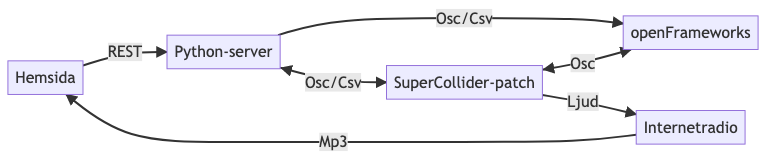
\includegraphics[width=0.5\textwidth]{../media/flowchart.png}
\caption{Översiktsdiagram av system}
\label{system}
\end{figure}

\subsection*{\gls{stack}}
\addcontentsline{toc}{subsection}{Stack}
För att driftsätta systemet valde jag att hyra en så kallad \gls{vps}, som tillåter mig att hyfast obegränsat installera, konfigurera och köra de program som jag behöver. Som operativsystem valde jag Ubuntu\footcite[version 20.04]{noauthor_enterprise_nodate}, eftersom det är det jag har installerat på min hemmaserver, som jag har använt under utvecklingsfasen av projektet. Som server till användargränssnittet använder jag Nginx\footcite{noauthor_nginx_nodate} och till Flask-API:et\footcite{noauthor_welcome_nodate} använder jag Gunicorn\footcite{noauthor_gunicorn_nodate}. SuperCollider, Darkice\footcite{noauthor_darkice_nodate}\footnote{Darkice används för att koda ljudströmmen till ett sändningbart MPEG-format.} och Icecast\footcite{noauthor_icecast_nodate}\footnote{Icecast används för att utsända, en. \emph{broadcast}, ljudströmmen till alla lyssnare.} har jag valt att köra samtliga som så kallade \emph{services}, vilket underlättar vid uppstart och omstart, utifall systemet eller någon del av det skulle krascha. Att de körs som \emph{services} underlättar också loggning, till exempel kan jag låta SuperCollider skriva ut viktiga händelser som tidpunkten när ett nytt datapaket mottagits av programmet. Dessa utskrifter har jag senare åtkomst till via Unix-kommandot \texttt{journalctl}.


\begin{figure}[H]
\centering
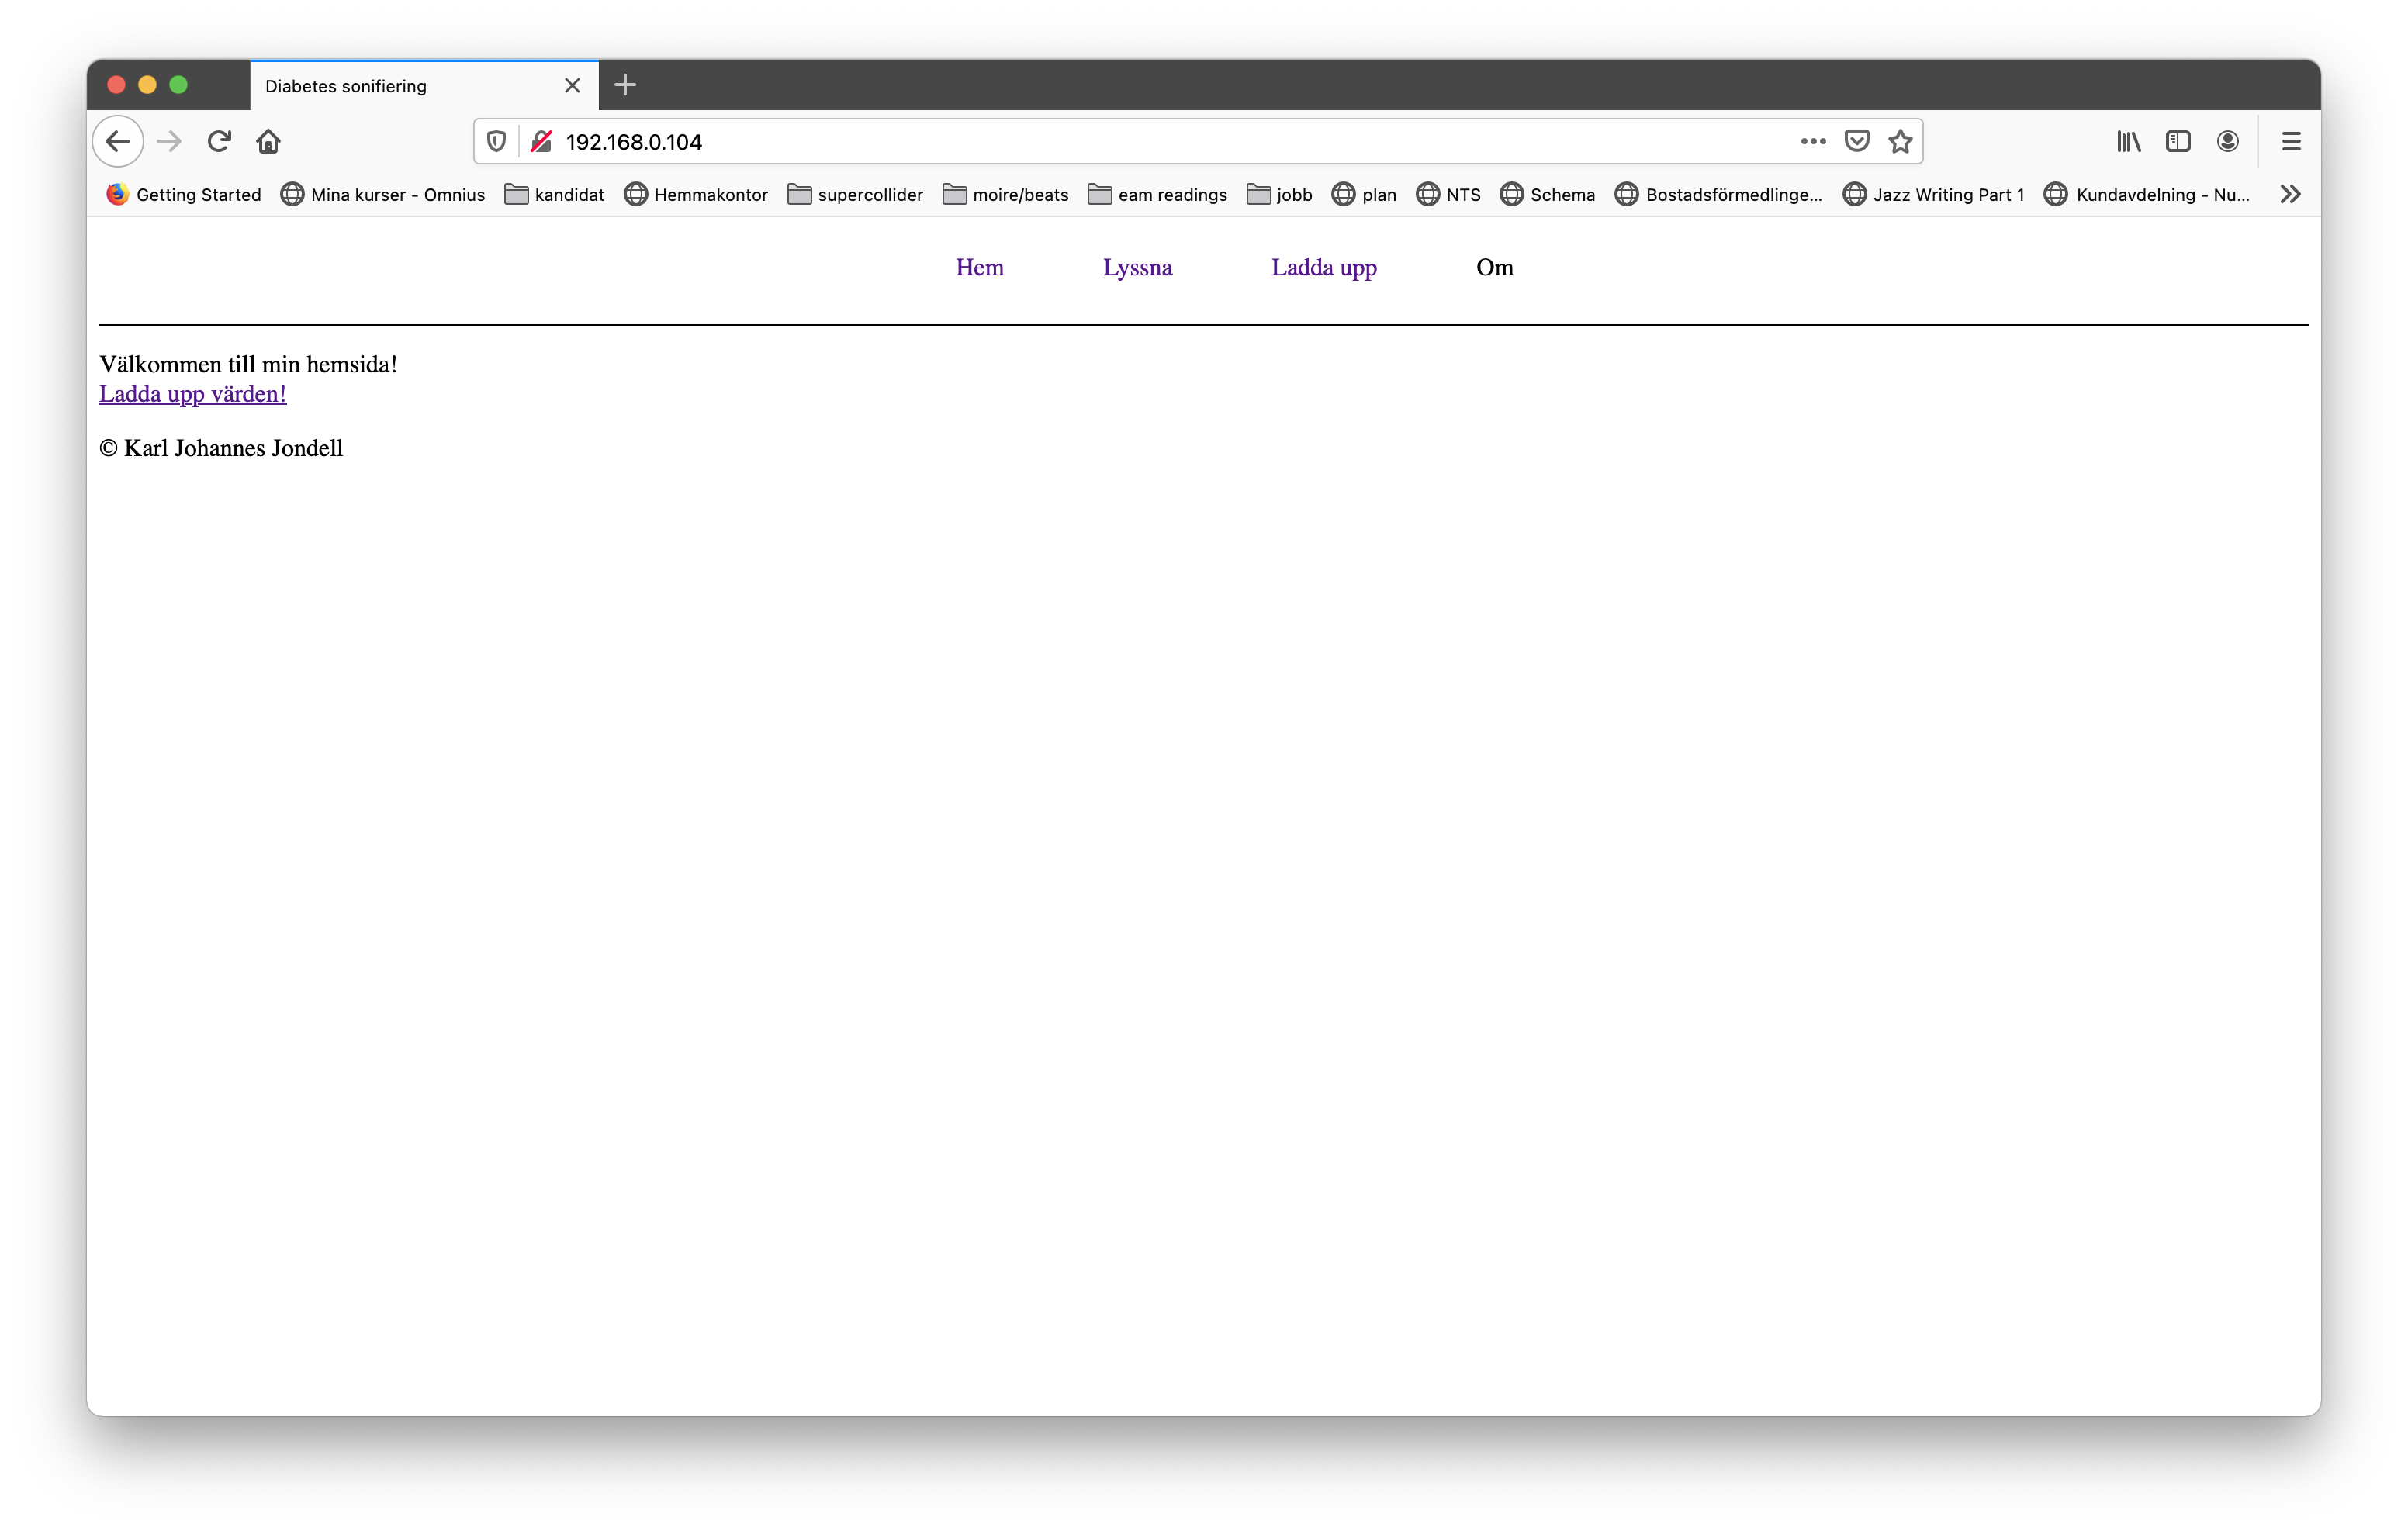
\includegraphics[width=\textwidth]{../media/hemsida.png}
\caption{Skärmdump av hemsida (\emph{temporär})}
\label{hemsida}
\end{figure}


\subsection*{Webbplats}
\addcontentsline{toc}{subsection}{Webbplats}
Webbplatsen finns tillgänglig på domänen\footcite{jondell_radio_nodate}: \url{https://radiodiabetes.eu/}. I figur \ref{hemsida} ovan visas en skärmdump av webbplatsen tagen den 13 april 2021.

Många webbplatser är uppdelade i en \emph{front end} och en \emph{back end}, och nedan följer en redogörelse av hur jag implementerat dessa för \emph{Radio Diabetes}. 

\subsubsection*{\gls{frontend}}
\addcontentsline{toc}{subsubsection}{\emph{Front end}}
För att bygga webbplatsens \emph{front end}, som jag fick hjälp av min vän Herman Wikner med, använde jag ett JavaScript-bibliotek som heter React.js\footcite{noauthor_react_nodate}. Webbplatsen består huvudsakligen av tre undersidor med information, en plats för att ladda upp filerna, och en kontrollmeny till radion, där besökaren kan spela och pausa musiken. Jag ville att musiken skulle spelas oavbrutet när en besökare navigerar på webbplatsen, och det var en av huvudanledningarna till att jag valde att använda React.js istället för endast HTML och CSS. Överlag ville jag ha en så smärtfri så kallad \gls{ux} som möjligt, för att göra deltagandet så enkelt som möjligt och för att göra installationen så tillgänglig som möjligt. I slutändan är det musiken som ska stå i fokus.

Kommunikationen till Flask-API:et sker via HTTP-metoderna \texttt{POST} och \texttt{GET}, där React.js skickar filinnehållet till Flask-API:et via \texttt{POST}-metoden, och får tillbaka ett svar om filen överförts utan problem eller inte.

%Själva gränssnittet är egentligen inte särskilt avancerat --- egentligen består det bara av tre olika sidor med mestadels text, en plats för att ladda upp filerna, och en radiospelare --- men eftersom jag ville ha 

% TODO få med "jag ville göra en så smärtfri ux som möjligt, för att göra deltagandet så enkelt som möjligt, tillgänglighet. musiken i fokus.

\subsubsection*{\gls{backend}}
\addcontentsline{toc}{subsubsection}{\emph{Back end}}
Behovet av ett så kallat \gls{api} kommer av att jag behövde en mellanhand för att överföra informationen från de uppladdade filerna till mitt SuperCollider-prpgram. Från tidigare experiment med mina blodsockervärden hade jag redan byggt ett Python-program\footcite{jondell_kj-jondelldiabetes-synth_2021} för att extrahera mätvärden från de Excel-filer som man kan exportera från Diasend. Därför återanvände jag en del av denna kod, och omstrukturerade denna för att kunna köras som ett \gls{flask}-program\footnote{Flask är ett webbramverk för Python. Det går alltså att använda Python-kod i Flask.}. När \gls{api}:et tar emot filinnehållet från användargränssnittet via \texttt{POST}-metoden så skapar den direkt två listor bestående av inlästa tidsvärden och blodsockervärden från filen. Filen sparas alltså aldrig på servern. \gls{api}:et gör också en del felhantering genom att försäkra att datavärdena är formaterade på ett korrekt sätt, i mmol/L, och att de är inom det möjliga intervallet. Sedan skickar det vidare listorna med värden till SuperCollider-programmet, via Osc. 

Sammanfattningsvis har alltså \gls{api}:et tre huvudsakliga funktioner: att tolka\footnote{I den mening som en \emph{parser} tolkar.} de delade filerna, felhantera korrupta filer eller korrupt data, och upprätta en Osc-kommunikation med SuperCollider.
%\begin{figure*}[H]
%\centering
%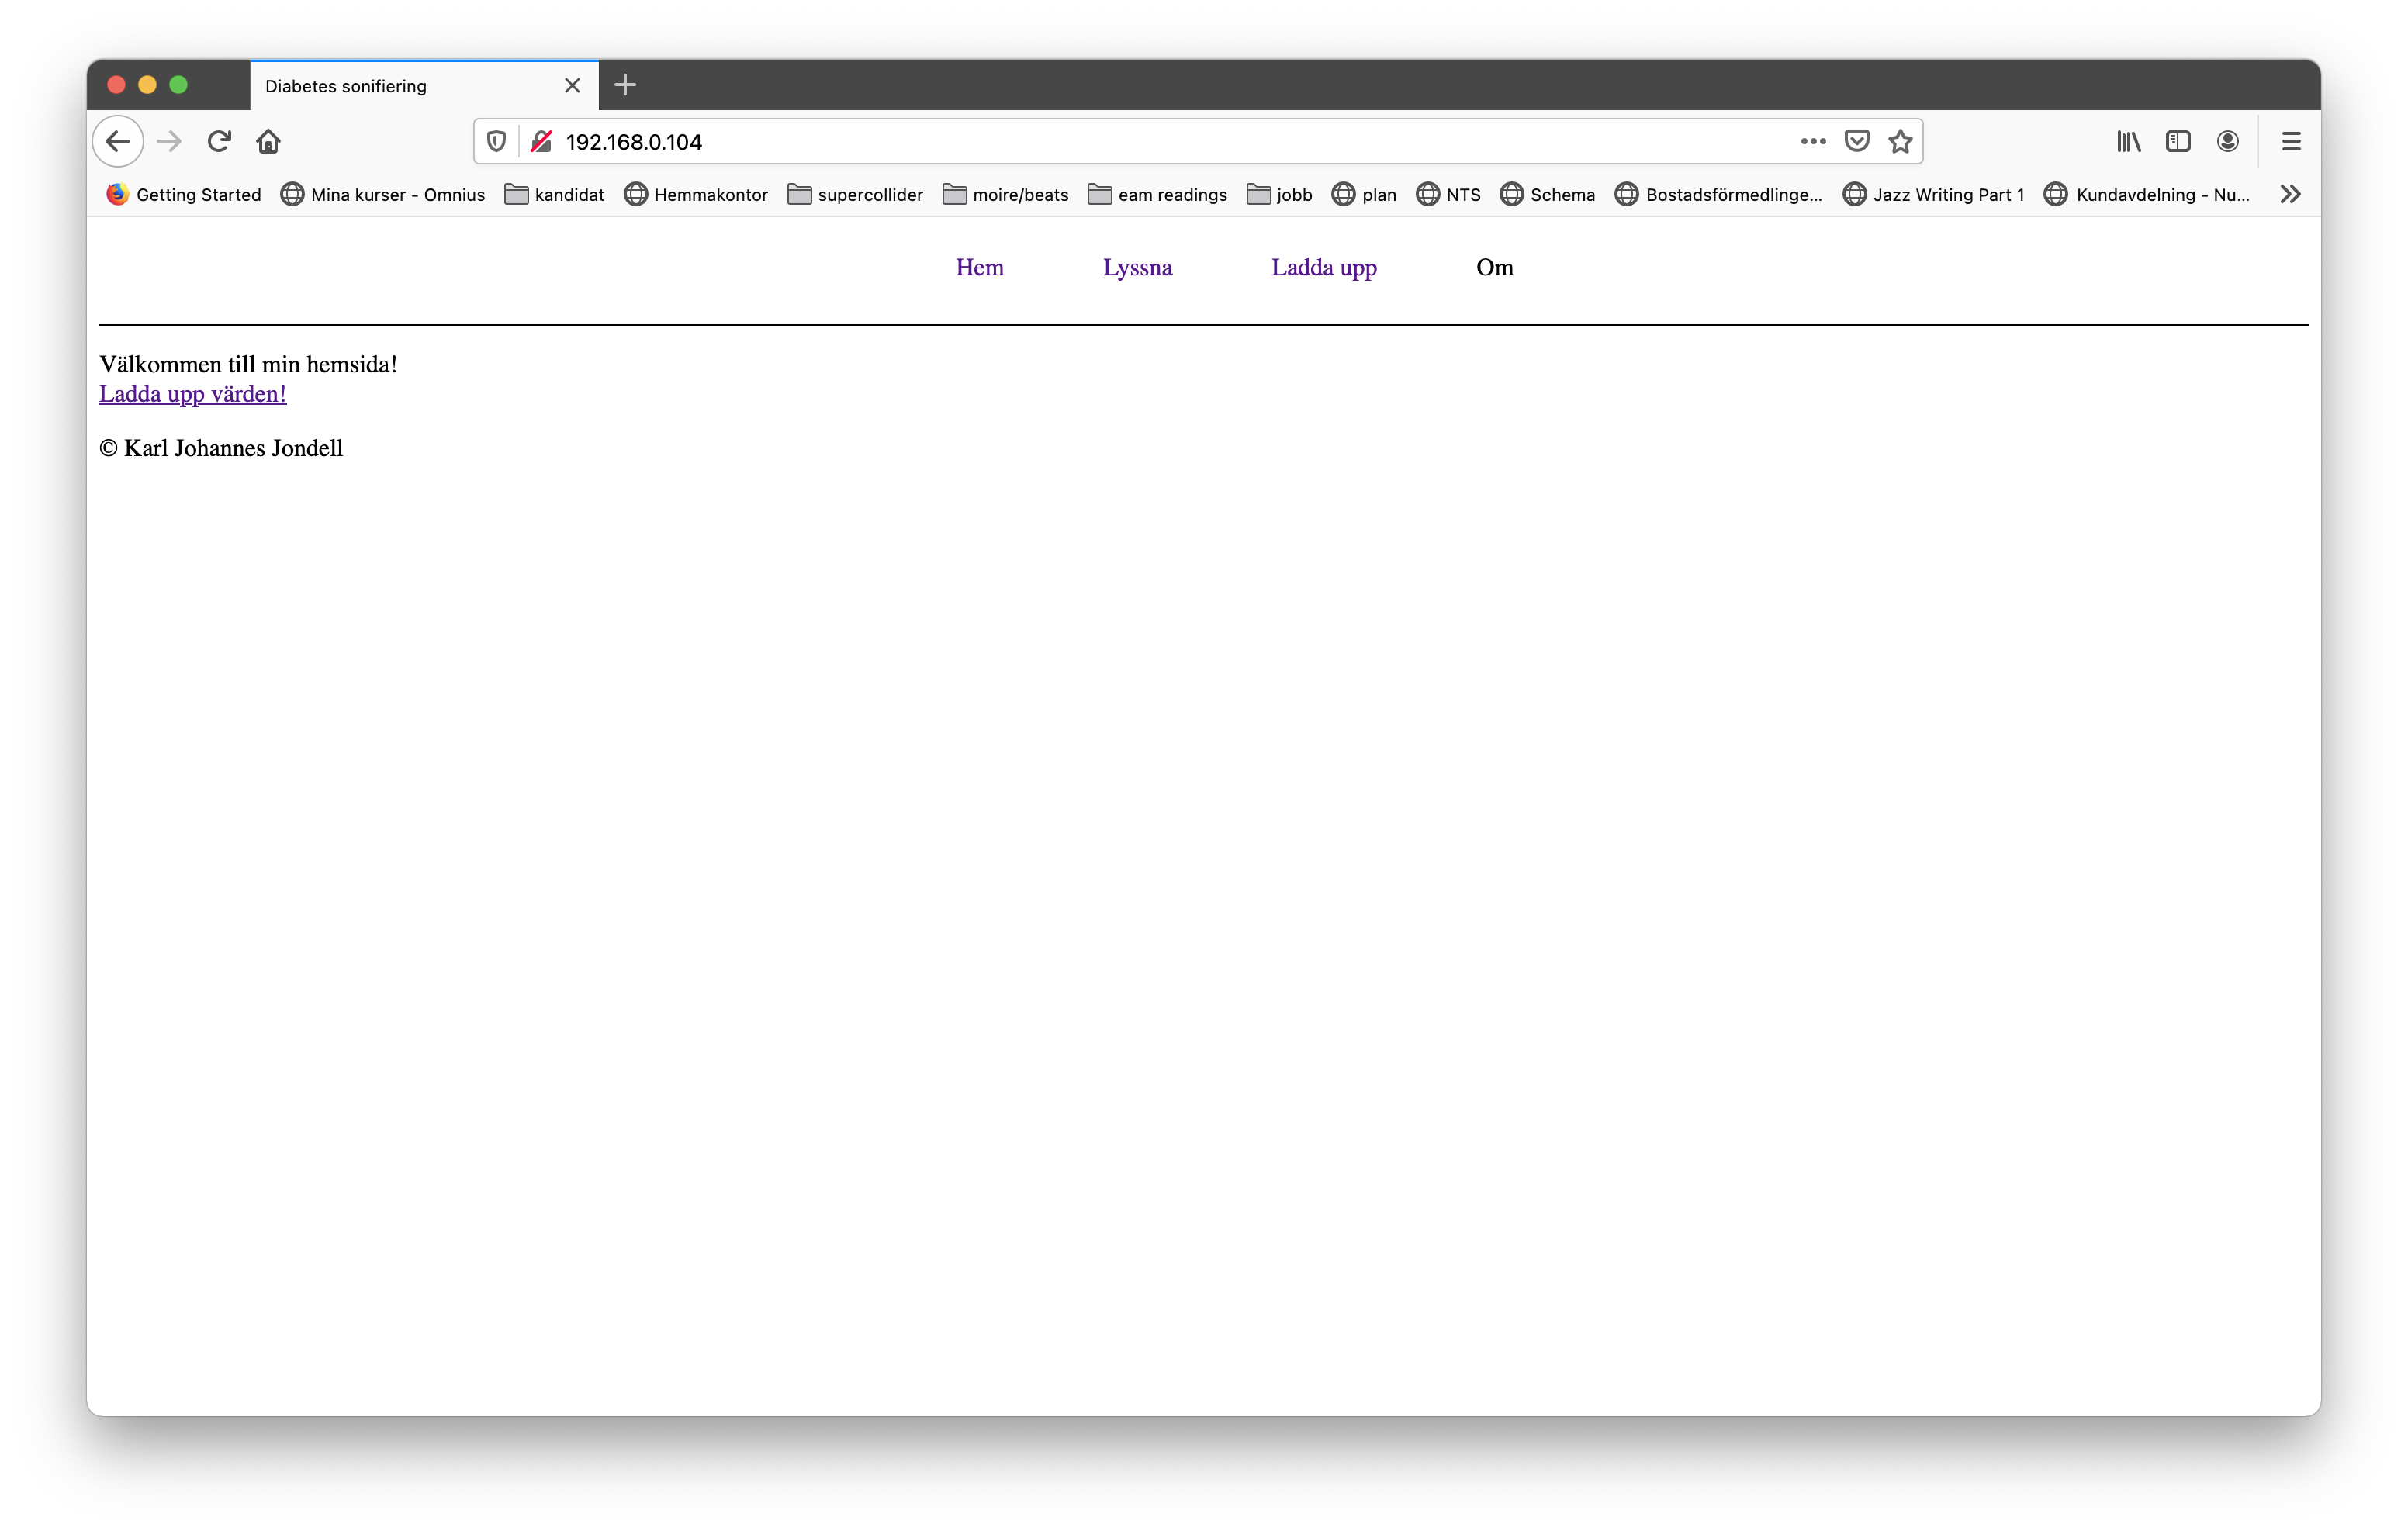
\includegraphics[width=\textwidth]{../media/hemsida.png}
%\caption{Skärmdump av hemsida (\emph{temporär})}
%\label{hemsida}
%\end{figure*}


\subsection*{SuperCollider-system}
\addcontentsline{toc}{subsection}{SuperCollider-system}
När en deltagare laddar upp en fil med sina mätvärden så skickas de vidare, via Flask-API:et, till \gls{supercollider}-programmet, som spelar upp en tack-hälsning för att ge en direkt återkoppling till deltagandet. Varje instans av mätdata --- det vill säga varje interaktion med installationen --- gestaltas av en specifik musikalisk funktion, för att på sätt ge deltagaren en koppling och förståelse till hur dennes bidrag påverkar musiken. 
I SuperCollider-programmet representeras varje sådan instans av mätdata av ett \emph{objekt}, som innehåller attribut som bland annat: register, skala, speltid, panorering, klangkälla/\gls{synthdef}, och tillhörande {\gls{pattern}}. Dessa attribut är antingen direkt bestämda av mätdatan --- en så kallad \emph{mappning} --- eller bestämda utifrån de andra aktiva objekten, till exempel redan upptagna register. Skapandet av dessa objekt gör programmet så fort det mottagit ett nytt paket av mätdata från Flask-API:et. Samtidigt avgör programmet om objektet ska spelas upp direkt, eller om det ska läggas på kö. 

\subsubsection*{Kösystemet}
\addcontentsline{toc}{subsubsection}{\emph{Kösystemet}}
Behovet av ett kösystem kommer ur scenariot att flera deltagare laddar upp värden inom en relativt kort tidsram. Om detta händer \emph{utan ett kösystem}, kan systemet reagera på två sätt: antingen spelas alla objekt upp samtidigt, med risk för att överrösta varandra och bli en kakofoni, eller så ersätter de varandra, vilket skulle leda till att ens bidrag inte skulle höras mer än en väldigt kort stund. En kompromiss är att använda ett kösystem, så att antalet samtidigt spelande objekt begränsas, och att dessa spelas \emph{minst} en given längd tid, men inte längre än en annan bestämd tid, om det står väntande deltagare på kö. Allt som allt har jag begränsat antalet samtidigt spelande objekt till \emph{tre} stycken, och när dessa är fyllda ställs antingen ett nytt bidrag på kö --- om inte de spelande objekten har varit aktiva i den givna minimumtiden --- eller så ersätter det nya bidraget det äldsta spelande objektet. Kösystemet är i tekniska termer alltså ett \gls{fifo}-system.


\subsection*{Tillvägagångssätt}
\addcontentsline{toc}{subsection}{Tillvägagångssätt}
Eftersom jag har byggt ett hyfsat komplext system, med många av varandra beroende delsystem, har jag stött på en del oförutsägbarheter under resans gång, något jag vill reflektera över här.

En förutsättning till att jag skulle få allt att fungera var att utveckla systemet modulärt, det vill säga att de olika beståndsdelarna (se diagram i i figur \ref{system} för referens) är fristående, med in- och utdata som passerar genom dem. För mig har själva SuperCollider-programmet alltid varit en central och prioriterad del av hela systemet, då det är den som faktiskt genererar musiken som jag har komponerat, och därför började jag med att bygga det. Till en början lät jag programmet använda en hårdkodad lista med mätvärden som indata, då jag inte hade byggt färdigt webbplatsen och API:et. Detta påverkade mina konstnärliga val i SuperCollider, eftersom jag hade ganska lite variation i mätvärdena. Jag hade heller inte bestämt några begränsningar i vad mitt SuperCollider-program skulle generera för musik, och frihetsgraden var väldigt hög, så det var svårt att veta hur mycket tid jag skulle lägga på den delen, och jag hade också svårt att känna mig nöjd. I slutändan bestämde jag mig för att utveckla delarna parallellt istället för sekvensiellt.

Just utvecklingen av webbplatsen och programmeringen i React.js och Flask blev kanske den största flaskhalsen i projektet, och det mycket på grund av att jag aldrig byggt en dynamisk webbapplikation tidigare. I planeringsfasen hade jag lite svårt att bestämma mig för vilken sorts arkitektur jag skulle använda mig av --- en enklare sida med endast Flask, CSS och HTML, eller React.js och Flask --- och det var ett ganska sent beslut som jag tog att faktiskt använda React.js, som medförde många fördelar med \gls{ux} i åtanke, men som samtidigt blev en tidskrävande omställning. Just planeringsmässigt tror jag att projektet lidit av att jag dels haft väldigt svårt att avgöra hur lång tid saker skulle ta, att jag inte heller vetat hur många timmar jag haft till förfogande, att jag inte haft tydliga milstolpar och mål, att jag kanske varit för ambitiös. Genomföringsmässigt har det också lidit av mitt vacklande självförtroende och en gnutta utmattning. Eftersom det är ett konstnärligt projekt så tror jag det kanske är omöjligt att formulera tydligare mål och milstolpar än de jag haft, men jag har samtidigt haft en känsla av att jag lätt fastnat i detaljer. 

En mot detta motstridig erfarenhet som jag hade med utvecklingen av SuperCollider -programmet var att jag hade en ganska stark idé om att inte göra ``enkla'' \emph{en-till-en} mappningar av mätvärdena till tonhöjd. Det var en väldigt kontraproduktiv idé, rotad i ambitionen av att musiken inte skulle bli transparent och avslöjande om de bakomliggande värdena. När jag väl provade att göra den mappningen så var effekten väldigt annorlunda: jag tyckte inte alls att det var för transparent, eller ens tråkigt, jag gillade hur det lät. Utan att bli allt för efterklok och självkritisk så önskar jag ändå att jag inte hade haft så många förutfattade meningar om hur musiken i slutändan skulle låta.

\section*{Musiken}
\addcontentsline{toc}{section}{Musiken}

Musiken genereras av SuperCollider-programmet som jag har skrivit. Jag har fyra olika instrument, eller musikaliska funktioner, tillgängliga:

  %\setlist{nolistsep}
  \begin{enumerate}[noitemsep]
	\item Ett fundament bestående av en GSM-avkodad formant-filtrerad ``kör''.
	\item Sinusvågor och elektroniska störningsljud som spelar rytmiska arpeggion.
	\item En wavetable-synth.
	\item Ett samplings-baserat slagverksliknande instrument.
  \end{enumerate}

Alla instrument som spelar arpeggion, det vill säga 2 och 4 i tabellen ovan, spelar i en pentatonisk durskala, där skalstegen bestäms av de inkommande mätvärdena. När de skapas tilldelas en transponering som bestämmer vilket omfång/register de ska spela i, samt en panorering i stereofältet. Viss variation i envelop och duration har jag skapat med en stokastisk variabel --- med andra ord en slumpgenerator --- men annars bestäms alla parametrar av mätvärdena. Att jag valde just att låta dem spela i en pentatonisk skala var för att jag ville ha en förhållandevis enkel harmonik och melodik, kontrasterat med vissa av de mer komplexa, hårda klangerna. 

Ljudmaterialet i de samplingsbaserade instrumenten har jag tagit från diverse inspelningar som jag har gjort genom åren: jag ville att de skulle ha en personlig koppling till mig. Den GSM-avkodade ljudfilen som utgör ``kören'' skapade jag av \emph{misstag} genom att läsa in en annan ljudfil som om den vore GSM-kodad i programmet Audacity. Effekten är en hård och övertonsrik klang, som jag låter passera genom ett formant-filter för att skapa en ljudkälla som påminner om människorösten. Denna ``kör'' sjunger en följd av fyra ackord, som upprepas utan variation. Däremot varieras andra parametrar av detta instrument, som duration och formant-vokal. De andra samplingarna jag använt är utklipp av elektroniska störningsljud --- återvunna från mitt förstaårsprojekt \emph{Calling out of context}\footcite{jondell_calling_2019}, men i ny tappning --- och en inspelning av min induktionshäll. Samtliga inspelningar som jag har använt har en viss \emph{elektrisk} karaktär, vilket blivit en stor del av min ljudpalett. 

Wavetable-synthen, det vill säga punkt nummer 3 i tabellen, är en sorts \gls{audification} av de inkommande mätvärdena. Dessa omvandlas till så kallade \emph{wavetables} som används av en \gls{ugen}\footnote{Som heter \texttt{VOsc3}.} i SuperCollider. På så sätt kan jag kontrollera tonhöjden samtidigt som klangfärgen helt bestäms av mätvärdena. Detta\footcite{jondell_kj-jondelldiabetes-synth_2021} är en \gls{synthdef} som jag utvecklat under en längre tid, men som jag anpassat till \emph{Radio Diabetes} för att direkt omvandla mätvärdena till wavetables. Tidigare har jag använt ett annat program för att göra själva omvandlingen, men det var inte möjligt för detta projekt, då det hade krävt att jag sparat ned värdena som ljudfiler. Eftersom jag inte velat spara värdena i någon form på min server var detta inte möjligt.

\subsection*{Rumslighet}
\addcontentsline{toc}{subsection}{Rumslighet}
Varje nyskapat objekt ges en unik position i stereofältet, och på så sätt en plats i rummet i musiken. 

Presentationen av radioströmmen genom webbplatsen som jag har utformat påverkar också den upplevda rumsligheten i musiken, där webbplatsen blir en visuell representation av rummet. Denna virtuella och visuella rumslighet som uppstår via webbplatsen blir den enda gemensamma nämnaren för besökarna, som kan befinna sig på helt olika fysiska platser vid själva lyssningen.

Ett planerat konserttillfälle kommer att ske den 20 maj i Lilla Salen på Kungliga Musikhögskolan. Då spelas ett utdrag ur radioströmmen upp, som den hörs i realtid. I och med de rådande restriktionerna så kommer ingen publik kunna närvara, utan konserten strömmas vidare till en publik i etern. Själva konserttillfället blir därför en sorts manifestation av radioströmmen i tid och rum.


\subsection*{Temporalitet}
\addcontentsline{toc}{subsection}{Temporalitet}
\emph{Radio Diabetes} utspelar sig --- i sin helhet --- någonstans mellan de tidsskalor som Curtis Roads i sin bok \emph{Microsound}\footcite{roads_microsound_2004} benämner \emph{infinite} och \emph{supra}, den senare definierar Roads som: \say{A time scale beyond that of an individual composition and extending into months, years, decades and centuries}\footcite[3]{roads_microsound_2004}. Eftersom min installation spelas upp i en radiosänding, vill jag undvika \emph{radiotystnad}, och ett konstnant flöde av musik strömmas därför ut. Utan tystnaden som markör för en början eller slut blir lyssnandet fokuserat på skeenden i \emph{nuet}. Varje lyssnare hamnar \emph{in media res} i musiken när de klickar på spela-knappen, i en unik start- och stoppunkt i musikens skeenden, men befinner sig samtidigt i samma \emph{nu} som de andra besökarna som för tillfället besöker webbplatsen. En besökare som också laddar upp sina värden kommer ha ytterligare en annan tidsuppfattning, då denne kanske väntar på att höra sitt bidrag: som antingen spelas upp direkt eller ställs i kö.

Roads beskriver\footcite[13]{roads_microsound_2004} hur \emph{macroform} kan uppstå på två sätt: det ena kallar han \emph{top-down} och det andra \emph{bottom-up}. I \emph{Radio Diabetes} bestäms denna form av de underliggande processer som utgör musiken, och därför är den ett exempel av \emph{bottom-up}. 
%En ambition jag haft har varit att tidsbestämma olika möjliga skeenden. Med andra ord, att musiken påverkas av tiden på dygnet, till exempel att vissa instrument spelas endast under vissa timmar, eller dagar. Då skulle jag möjligtvis behöva förhålla mig till en \emph{top-down}-metod, att planera ut när vissa saker skulle hända, eller i vilken ordning. Men detta är än så länge bara en framtida eventualitet.

\subsection*{Generativitet och interaktivitet}
\addcontentsline{toc}{subsection}{Generativitet och interaktivitet}
I texten \emph{Defining Sound Toys: Play as Composition}\footcite{collins_defining_2014} beskriver Dolphin en form av interaktivt, audiovisuellt kompositionssystem som han kallar \emph{sound toys}. \emph{Sound toys} bjuder in till en högre grad av lekfullhet och fritt interagerande och reagerande än vad jag gör i \emph{Radio Diabetes} --- och därför kanske inte min installation klassificeras som en sådan --- men Dolphins text är ändå högst relevant för mitt projekt. Dolphin refererar bland annat till Umberto Ecos text \emph{The Poeitcs of the Open Work}, och hur det han kallar \emph{sound toys} faller in någonstans i gränslandet\footcite[53]{collins_defining_2014} mellan \emph{open work}, \emph{kompositionsverktyg} och \emph{instrument}. På många sätt existerar även mitt \emph{Radio Diabetes} i gränslandet mellan dessa tre kategorier, där \emph{instrument} möjligtvis går att byta ut mot \emph{en samling instrument} eller \emph{orkester}. 

För att återkoppla till Luciers kommentar om sitt stycke \emph{Music for Solo Performer} --- att form och struktur ska bestämmas av det bakomliggande \emph{naturliga} fenomenet, just för att det är \emph{naturligt} --- så har jag styrt och formaliserat musiken till en högre grad än vad Lucier gjorde, genom att göra strikta mappningar och bestämt hur mätvärdena \emph{får} gestaltas. Jag kanske har haft ett annat fokus och ambition med \emph{Radio Diabetes} än vad Lucier hade med sitt stycke, men för mig har det varit viktigt att försöka kontrollera det estetiska resultatet av min komposition, och försöka styra det till något som \emph{jag} tycker låter bra. I förlängningen hoppas jag då att även andra ska tycka det låter bra, och bli engagerade i projektet och nyfikna på att dela med sig. Eftersom det är en kollektiv ansträngning vill jag att så många som möjligt ska känna en glädje i att delta, men också att resultatet är estetiskt givande. %Från mitt förstaårsprojekt \emph{Calling out of context}\footcite{jondell_calling_2019} lärde jag mig att begränsa deltagandet, då jag upptäckte att det 

\section*{Slutsatser}
\addcontentsline{toc}{section}{Slutsatser}
Som tidigare nämnt var en ambition med detta projekt att uppmuntra delandet av blodsockervärden utan att de på något sätt värderas, att många diabetiker --- inklusive jag själv --- har ett behov av att dela sina värden med andra och känna en gemenskap och en trygghet. Eftersom \emph{Radio Diabetes} ännu inte formellt lanserats --- den 12 maj ska jag officiellt publicera och marknadsföra webbplatsen --- har jag inte fått någon återkoppling på andra diabetikers upplevelse av installationen. Men min förhoppning är att den kommer mottas med nyfikenhet. Min förhoppning är också att det estetiska resultatet som kommit av mitt kompositionsarbete lever upp till mina egna förväntningar. Det kan jag utvärdera först efter \emph{Radio Diabetes} är officiellt lanserat.

En av de främsta slutsatser jag dragit av att arbeta med detta projekt är att \emph{saker tar längre tid än vad jag hade tänkt}\footnote{Även känt som \emph{Hofstadters lag}.}. I planeringsfasen hade jag många idéer, och en stark motivation och ambition, som under projektets gång tyvärr dalat. Jag hade en vision om hur saker skulle låta, och hur de skulle fungera, men av många anledningar --- kanske främst att \emph{saker inte blir som man tänkt} --- så har jag varit tvungen att omforma stora delar av projektet. Men jag vill understryka att även om jag kanske varit ``för'' ambitiös eller ivrig, så är jag väldigt nöjd med att ha byggt en infrastruktur och arkitektur, en grund till plattformen, som jag i framtiden kan fylla med flera av mina musikaliska idéer. Nedan följer en redogörelse av vad jag hoppas kunna lägga till i framtiden till projektet.

\subsection*{Utvecklingsmöjligheter}
\addcontentsline{toc}{subsection}{Utvecklingsmöjligheter}
  \begin{enumerate}
	\item Jag hade en tanke om att göra det möjligt för deltagare att lämna meddelanden, antingen i formen av en gästbok på webbplatsen eller att sätta upp ett telefonnummer dit man kunde ringa och lämna meddelanden som spelas upp i radion. I det senare fallet ville jag uppmuntra delandet av upplevelser kring att leva med diabetes.
	\item En teknisk ambition jag har är att sätta upp två parallella radioströmmar, som jag kan växla mellan när jag vill underhålla och/eller utveckla SuperCollider-programmet. Som systemet fungerar nu måste jag stänga av radion för att göra förändringar i SuperCollider, något som skapar \emph{radiotystnad}. Med två parallella strömmar kan jag slussa lyssnarna till den ena medan jag jobbar på den andra.
	\item Rent rumsligt hade jag också en idé om att på något sätt binauralisera musiken --- kanske med hjälp av en generaliserad HRTF --- vilket skulle försätta lyssnaren i ett gemensamt akustiskt virutellt rum. Likt föregående punkt hade det kunnat möjliggöras genom att använda två strömmar, där den ena är binauraliserad och den andra vanlig stereo.
	\item Jag vill internationalisera webbplatsen genom att erbjuda en engelsk översättning av all text och bjuda in diabetiker från hela världen att delta. I praktiken är det redan idag möjligt för diabetiker utanför Sverige att delta, så länge deras sjukvårdsystem använder Diasend. Men ett möjligt problem är att vissa länder, som tidigare nämnt, inte använder samma mätenhet.
	\item Jag påbörjade ett försök att också visualisera delade mätvärden, med ett program som jag skrev i \emph{openFrameworks}. Själva programmet blev jag klar med, men att inkludera \emph{openFrameworks}-programmet i den infrastruktur jag byggde upp blev för tidskrävande och därför sköt jag upp den idéen. 
	\item Jag hade en ambition om att tidsbestämma olika \emph{möjliga} skeenden i musiken. Med andra ord, att musiken påverkas av tiden på dygnet, till exempel att vissa instrument spelas endast under vissa timmar, eller dagar.
  \end{enumerate}

%\clearpage
%\defbibfilter{internet}{
%  type=online or
%  type=misc
%}
\defbibfilter{litteratur}{
  type=book or
  type=incollection or
  type=article or
  type=thesis
}

\addcontentsline{toc}{section}{Referenser}
\printbibheading
\printbibliography[type=online,title={Internet},heading=subbibintoc]
\printbibliography[filter=litteratur,title={Litteratur},heading=subbibintoc]
\begin{refcontext}[sorting=mysort]
  \printbibliography[type=audio,title={Musik},heading=subbibintoc]
\end{refcontext}
\printbibliography[type=misc,title={Radio},heading=subbibintoc]

\clearpage
\begin{appendices}
\printglossaries
\end{appendices}


\subsection*{\emph{Radio Diabetes} (2021)}
\addcontentsline{toc}{subsection}{\emph{Radio Diabetes} (2021)}
Ett inspelat utdrag från själva radioströmmen, detsamma som spelades upp i Lilla Salen, är bifogat med denna text. Inspelningen skedde den 20 maj 2021.

\end{document}
